% ==============================================================================
% 第四章 有限機率空間
% ==============================================================================
\section{有限機率空間}\label{sec:b5-ch4}

\begin{center}
\begin{minipage}{0.75\textwidth}
\begin{itemize}[leftmargin=2em, itemsep=0.3em]
  \item[§ IV-1] \textbf{機率空間}
  \item[§ IV-2] \textbf{條件機率與獨立事件}
  \begin{itemize}[leftmargin=1.5em, itemsep=0.2em]
    \item[甲、] 條件機率
    \item[乙、] 貝氏定理
    \item[丙、] 獨立事件
  \end{itemize}
  \item[附錄] \textbf{一般機率空間的定義}
\end{itemize}
\end{minipage}
\end{center}

\begin{center}
$* \qquad * \qquad * \qquad * \qquad *$
\end{center}

在前一章中我們討論機會均等的機率，導出若干基本性質，並舉例說明機率的求法．但是對於機會不均等的問題，例如投一枚不公正的銅錢，就無法用 第三章的直觀機率來討論．因此我們需要將機率概念擴大才能解決此類問題．在本章中我們將討論一般的有限機率空間，亦卽有限的樣本空間，但不限定其中基本事件出現的機會均等．

% ==============================================================================
% § IV-1 機率空間
% ==============================================================================
\subsection{機率空間}\label{sec:b5-4-1}

由直觀認定機會均等而定義的古典機率，將樣本空間 $S$ 中每一事件 $A$，卽 $S$ 的每一個子集，對應到一個實數 $P(A)$，也就是說，如果令 $\mathscr{F}$ 表示 $S$ 的所有子集的集合，則 $P$ 就是一個自 $\mathscr{F}$ 到實數 $\mathbf{R}$ 並且滿足若干性質的函數．因一般的機率必須為直觀機率的擴展，故也應該具有這些性質，因此我們就從這個觀點給予定義如下：

\medskip
\noindent\textbf{定義}\quad 設 $S$ 是一個有限的樣本空間，$\mathscr{F}$ 是 $S$ 的所有子集形成的集合，以及 $P$ 是一個自 $\mathscr{F}$ 到 $\mathbf{R}$ 的函數：
\[
P \colon \mathscr{F} \longrightarrow \mathbf{R}
\]
並且滿足下列條件：
\begin{enumerate}[label=\Roman*., itemsep=2pt, topsep=2pt]
  \item 對於任意事件 $A \in \mathscr{F}$，$0 \le P(A) \le 1$．
  \item $P(S) = 1$（全事件必然發生）．
  \item 若 $A, B \in \mathscr{F}$，則
  \[
  P(A \cup B) = P(A) + P(B) \Longleftrightarrow A \cap B = \phi \quad \text{（互斥事件的加法性），}
  \]
\end{enumerate}
則稱 $P$ 為 $S$ 上的\textbf{機率函數}，對於每個 $A \in \mathscr{F}$，$P(A)$ 就叫做事件 $A$ 的\textbf{機率}．一個樣本空間 $S$ 連同一個機率函數 $P$ 合稱為一個\textbf{機率空間}，記作 $(S, \mathscr{F}, P)$ 或簡記為 $(S, P)$．

\medskip
\noindent\textbf{〔注意〕}
\begin{enumerate}[label=\arabic*., leftmargin=2em, itemsep=0.3em]
  \item 這種利用公理，導出一般機率空間的方法是由 Kolmogorov 所首創．
  \item 互斥事件的加法性 III 在第三章直觀機率可以證得，但在一般的機率是無法證明的，必須將其列為公理，承認此一事實．
  \item 由 II 及 III 可導出 $P(\phi) = 0$（空事件為不可能）．
  \item 公理 III 中 $P(A \cup B) = P(A) + P(B) \Longrightarrow A \cap B = \phi$ 並不必要，但如此可由上式推得 $P(A) = 0 \Longrightarrow A = \phi$（取 $B = S$ 卽可推得），這表示樣本空間 $S$ 中沒有\phantomsection\label{note:b5-ch4-p116-meiyou}\footnote{【原書註記/校訂】：原書印作「這表示樣本空間 $S$ 中設有機率為 0 的非空事件」，依前句 $P(A) = 0 \Longrightarrow A = \phi$ 及後文「不可能發生的基本事件都被排除」、「在無限的情形就會有機率為 0 的非空事件」，「設有」顯為「沒有」之排版訛誤，茲予校訂．}機率為 0 的非空事件，換句話說，不可能發生的基本事件都被排除．我們只有在有限機率空間的情形可以這樣做，在無限的情形就會有機率為 0 的非空事件．
\end{enumerate}

機率函數定義在 $\mathscr{F}$，卽所有事件的集合上，因此各基本事件的機率皆已確定．由條件 III 可以推出事件 $A$ 的機率等於 $A$ 中各基本事件的機率的和，卽若設
\[
A = \{a_1, \dots\dots, a_k\},
\]
則
\[
P(A) = P(a_1) + \dots\dots + P(a_k);
\]
式中 $P(a_j)$ 為 $P(\{a_j\})$ 的簡寫．反之，如果我們只適當地規定各基本事件的機率，也可經由上式定義，得到一個機率函數〔註〕．

\medskip
\noindent\textbf{〔註〕}在有限樣本空間的情形，這兩種做法的意義完全相同，但是對於無限的樣本空間，情形卽不相同．例如在討論幾何機率時，各樣本點的機率皆等於 0，上式無法適用，此時要考慮樣本點的機率密度並且利用積分計算．

\medskip
在前一章中我們已經指出直觀機率的古典定義滿足若干基本性質，那些性質中包含了現在機率函數定義中的三個條件，因此在前一章中所討論的例子實際上都是機率空間的特別情形，下面我們再舉幾個其他的例子．

\medskip
\noindent\textbf{【論例 1】}
\begin{enumerate}[(i), leftmargin=2em, itemsep=0.3em]
  \item 袋中有 3 紅球，2 白球，如任取一球（各球被取到機會均等），試寫出此試驗之機率空間．
  \item 將 (i) 中球數改為 5 紅球，3 白球．
\end{enumerate}

\indent\textbf{解}\quad
\begin{enumerate}[(i), leftmargin=2em, itemsep=0.3em]
  \item 樣本空間為 $S = \{\text{紅}, \text{白}\}$．令 $A = \{\text{紅}\}$ 表示取得一紅球的事件，$B = \{\text{白}\}$ 表示取得一白球的事件．則 $\mathscr{F} = \{\phi, A, B, S\}$ 機率函數為
  \[
  P(\phi) = 0,\quad P(A) = \frac{3}{5},\quad P(B) = \frac{2}{5},\quad P(S) = 1.
  \]
  容易證明滿足機率函數定義中的條件：I, II, III，卽 $(S, \mathscr{F}, P)$ 為機率空間．

  \item 設樣本空間 $S$ 及事件 $A, B$ 同上．此時機率函數為
  \[
  P(\phi) = 0,\quad P(A) = \frac{5}{8},\quad P(B) = \frac{3}{8},\quad P(S) = 1.
  \]
\end{enumerate}
（各事件之機率可由直觀看出並請參考以下論例 2 之討論）

這個例子說明在同一個樣本空間上可以作出不同的機率函數，因而構成不同的機率空間．在這個例子中，我們還是依照抽出機會均等的假設而導出機率函數，實際上如果我們不顧袋中的球數，隨意指定事件 $A, B$ 的機率，例如 $P(A) = P(B) = 1/2$，也可以得到一個機率函數，但是這樣將與實際經驗有很大偏差，不能應用．當然我們希望所討論的機率，能與日常經驗或實驗結果符合，才能達到實際應用的目的．

\medskip
\noindent\textbf{【論例 2】}
\begin{enumerate}[(i), leftmargin=2em, itemsep=0.3em]
  \item 同時擲三枚公正的硬幣，試寫出機率空間．
  \item 將三個相同的球任意分配在黑、白兩個箱中，試寫出機率空間．
\end{enumerate}

\indent\textbf{解}\quad
(i) 我們先將三枚硬幣編為 1, 2, 3 號，則有 8 種可能現象，每個現象的機率為 1/8．然後再將有關現象合併成基本事件，同時亦得到各基本事件的機率，如下表所示：

\begin{center}
\renewcommand{\arraystretch}{1.2}
\begin{tabular}{cccc|lc}
\hline\hline
1 & 2 & 3 & 機率 & 基本事件 & 機率 \\
\hline
正 & 正 & 正 & $1/8$ & \hphantom{$\Big\}$} 三個正 & $1/8$ \\
正 & 正 & 反 & $1/8$ & \multirow{3}{*}{$\left.\begin{array}{c} \vphantom{A}\\ \vphantom{A}\\ \vphantom{A}\end{array}\right\}$ 二正一反} & \multirow{3}{*}{$3/8$} \\
正 & 反 & 正 & $1/8$ & & \\
反 & 正 & 正 & $1/8$ & & \\
正 & 反 & 反 & $1/8$ & \multirow{3}{*}{$\left.\begin{array}{c} \vphantom{A}\\ \vphantom{A}\\ \vphantom{A}\end{array}\right\}$ 一正二反} & \multirow{3}{*}{$3/8$} \\
反 & 正 & 反 & $1/8$ & & \\
反 & 反 & 正 & $1/8$ & & \\
反 & 反 & 反 & $1/8$ & \hphantom{$\Big\}$} 三個反 & $1/8$ \\
\hline
\end{tabular}
\end{center}

(ii) 這個問題實際上與 (i) 相同．如果令 $x$ 表示黑箱中球數，$y$ 表示白箱中球數，寫作 $(x, y)$，則得基本事件及所求機率如下：
\begin{align*}
P \colon (3, 0) &\longrightarrow 1/8, \\
(2, 1) &\longrightarrow 3/8, \\
(1, 2) &\longrightarrow 3/8, \\
(0, 3) &\longrightarrow 1/8. \tag*{\#}
\end{align*}

\medskip
\noindent\textbf{〔例 1〕} 設同時擲公正的骰子三粒，試求此試驗的機率空間，如果令 $A$ 表示三粒出現相同點數的事件，試求 $A$ 的機率．

\indent\textbf{解}\quad 樣本空間可寫為
\[
S = \{(x, y, z) \mid x, y, z = 1, 2, 3, 4, 5, 6 \text{ 且 } x \le y \le z\},
\]
仿照論例 2 的討論則基本事件的機率為：
\[
P(x, y, z) = \begin{cases}
\dfrac{6}{216} & \text{對於 } x < y < z, \\[8pt]
\dfrac{3}{216} & \text{對於 } x = y < z \text{ 或 } x < y = z, \\[8pt]
\dfrac{1}{216} & \text{對於 } x = y = z
\end{cases}
\]
（有時為了清楚起見，機率函數也用 $P[\quad]$ 表示），事件
\[
A = \{(x, x, x) \mid x = 1, 2, 3, 4, 5, 6\}. \text{ 因此}
\]
\[
P(A) = \frac{6}{216} = \frac{1}{36}.
\]

\medskip
\noindent\textbf{注意}\quad 例 1 中樣本空間有 56 個樣本點，論例 2 中各有 4 個樣本點，我們不能直接按照機會均等原則指定各樣本點有相同機率．

由機率函數定義中的條件，我們也可以推得一些其他的性質．

\medskip
\noindent\textbf{【定理 1】}若 $A_1, A_2, \dots\dots, A_k \in \mathscr{F}$ 為互斥事件，則
\begin{equation}
P(A_1 \cup \dots\dots \cup A_k) = P(A_1) + \dots\dots + P(A_k) \label{eq:b5-ch4-1}
\end{equation}
證明與第三章 §III-1 之 ($\text{IV}'$) 相同，故予省略．

\medskip
\noindent\textbf{【定理 2】}對於任意事件 $A \in \mathscr{F}$，餘事件 $A' = S - A$ 的機率為
\begin{equation}
P(A') = 1 - P(A) \label{eq:b5-ch4-2}
\end{equation}
對於任意二事件 $A, B \in \mathscr{F}$，和事件 $A \cup B$ 的機率為
\begin{equation}
P(A \cup B) = P(A) + P(B) - P(A \cap B) \label{eq:b5-ch4-3}
\end{equation}

\noindent\textbf{證明}\quad 因為 $A \cup A' = S$ 及 $A \cap A' = \phi$，所以
\[
1 = P(S) = P(A \cup A') = P(A) + P(A').
\]
設 $A, B$ 為任意二事件，我們有
\[
A = (A \cap B) \cup (A \cap B') \quad\text{及}\quad (A \cap B) \cap (A \cap B') = \phi,
\]
因此
\[
P(A) = P(A \cap B) + P(A \cap B').
\]
同理
\[
P(B) = P(A \cap B) + P(A' \cap B).
\]
將上二式相加得
\[
P(A) + P(B) = 2P(A \cap B) + P(A' \cap B) + P(A \cap B').
\]
但 $A \cap B,\, A' \cap B,\, A \cap B'$ 三者互斥且
\[
(A \cap B) \cup (A' \cap B) \cup (A \cap B') = A \cup B,
\]
由 (1) 式得
\[
P(A) + P(B) = P(A \cap B) + P(A \cup B). \tag*{\#}
\]

\medskip
\noindent\textbf{【系理】}設 $A, B \in \mathscr{F}$ 為任意事件，則
\begin{equation}
P(A \cup B) \le P(A) + P(B) \label{eq:b5-ch4-4}
\end{equation}
一般地，若 $A_1, A_2, \dots\dots, A_k \in \mathscr{F}$ 為任意事件，則
\begin{equation}
P(A_1 \cup \dots\dots \cup A_k) \le P(A_1) + \dots\dots + P(A_k) \label{eq:b5-ch4-5}
\end{equation}

\noindent\textbf{證明}\quad 由 (3) 式及 $P(A \cap B) \ge 0$ 卽得到 (4) 式．

(5) 式可利用數學歸納法證明：
\begin{align*}
P(A_1 \cup \dots\dots \cup A_k) &= P[(A_1 \cup \dots\dots \cup A_{k-1}) \cup A_k] \\
&\le P(A_1 \cup \dots\dots \cup A_{k-1}) + P(A_k) \\
&\le P(A_1) + \dots\dots + P(A_{k-1}) + P(A_k). \tag*{\#}
\end{align*}

由機率函數定義中的條件 III，我們還可以直接推得下列性質：

\medskip
\noindent\textbf{單調性：}若 $A, B \in \mathscr{F}$，且 $A \subset B$，則
\begin{equation}
P(A) \le P(B) \label{eq:b5-ch4-6}
\end{equation}

\noindent\textbf{非空事件的可能性：}若 $A \in \mathscr{F}$ 且 $A \neq \phi$，則
\begin{equation}
P(A) > 0 \label{eq:b5-ch4-7}
\end{equation}

(7) 式的意義表示我們所取的樣本空間 $S$ 是最經濟的，因為 $S$ 中沒有包含不可能的非空事件，但是如果將條件 III 改為：若 $A, B \in \mathscr{F}$，
\[
A \cap B = \phi \Longrightarrow P(A \cup B) = P(A) + P(B).
\]
我們卽不能導出 (7) 式，因此可在 $S$ 中摻入任意多個不可能的非空事件．

\medskip
\noindent\textbf{〔例 2〕} 擲一粒公正的骰子三次．設 $A$ 表示第一次出現 6 點的事件，$B$ 表示第二次出現 6 點的事件．試求和事件 $A \cup B$ 的機率．

\indent\textbf{解}\quad 和事件 $A \cup B$ 表示第一次或第二次出現 6 點的事件，積事件 $A \cap B$ 表示第一次及第二次皆出現 6 點的事件，因此
\begin{align*}
P(A \cup B) &= P(A) + P(B) - P(A \cap B) \\
&= \frac{1}{6} + \frac{1}{6} - \frac{1}{36} = \frac{11}{36}. \tag*{\#}
\end{align*}

\medskip
\noindent\textbf{〔例 3〕} 同時擲三粒公正的骰子，設 $A$ 表示恰有一粒 5 點的事件，$B$ 表示恰有一粒 6 點的事件，試求和事件 $A \cup B$ 的機率．

\indent\textbf{解}\quad 和事件 $A \cup B$ 表示恰有一粒 5 點或恰有一粒 6 點的事件，積事件 $A \cap B$ 表示恰有一粒 5 點及一粒 6 點的事件．因此
\begin{align*}
P(A \cup B) &= P(A) + P(B) - P(A \cap B) \\
&= \frac{25}{72} + \frac{25}{72} - \frac{1}{9} = \frac{7}{12}\phantomsection\label{note:b5-ch4-p121-calc}\footnote{【原書註記/校訂】：原書此處印作「$= \frac{25}{72} + \frac{25}{72} - \frac{1}{9} = \frac{31}{36}$」，經計算 $\frac{50}{72} - \frac{8}{72} = \frac{42}{72} = \frac{7}{12}$（約分前亦作 $\frac{21}{36}$），原書「$\frac{31}{36}$」顯為計算或排印訛誤，茲更正為 $\frac{7}{12}$ 並加註說明．}. \tag*{\#}
\end{align*}

對於擲硬幣，擲骰子，以及取球等這些類型的問題，我們由機會均等的假設推出各種事件的機率，而所得的結果也與經驗符合，所以能夠實際應用，但是在很多應用問題中，我們無法採取同樣的方式來討論，而要改用經驗的方法．我們對於所研究的對象作較長時期或較大規模的觀測，或者對於所進行的實驗作較多次數的重複，逐次記錄結果，加以分析整理，卽可對於其中各種可能出現事件給定相當程度準確的機率．例如設在某項試驗中所有可能出現的基本事件為 $\{a_1, a_2, \dots\dots, a_k\}$，而對於相當大的 $N$ 作 $N$ 次重複試驗中 $a_j$ 出現的次數為 $N_j$，$j = 1, 2, \dots\dots, k$，$N_1 + \dots\dots + N_k = N$．則我們可規定基本事件 $a_j$ 的機率為
\[
P(a_j) = \frac{N_j}{N}.
\]
在一般情況，這樣所得到的機率就能夠適合應用的需要．關於這一方面的詳細討論，屬於統計推測的範圍．

\medskip
\noindent\textbf{〔例 4〕} 孟德爾 (Mendel) 的豌豆試驗．

孟德爾在 1865 年選用第一代黃色雜交品種自行交配，試驗結果得黃色種子 75.05\%，綠色種子 24.95\%，與推出的遺傳定律 $3 : 1$ 非常接近．

\medskip
\noindent
\begin{minipage}[t]{0.62\textwidth}
\textbf{〔例 5〕} 某工廠生產真空管，經試驗 400 只之使用壽命如右表．
\begin{enumerate}[(i), leftmargin=2em, itemsep=0.3em]
  \item 試求使用壽命在 500 小時以下之機率．
  \item 試求使用壽命在 500 至 999 小時之機率．
  \item 試求使用壽命在 1000 小時以上之機率．
\end{enumerate}
\end{minipage}\hfill
\begin{minipage}[t]{0.35\textwidth}
\centering
\renewcommand{\arraystretch}{1.15}
\begin{tabular}{|c|c|}
\hline
\begin{tabular}{c} 使用壽命 \\ （小時） \end{tabular} & 個\quad 數 \\
\hline
$300\text{---}399$ & 14 \\
$400\text{---}499$ & 46 \\
$500\text{---}599$ & 58 \\
$600\text{---}699$ & 76 \\
$700\text{---}799$ & 68 \\
$800\text{---}899$ & 62 \\
$900\text{---}999$ & 48 \\
$1000\text{---}1099$ & 22 \\
$1100\text{---}1199$ & 6 \\
\hline
合\qquad 計 & 400 \\
\hline
\end{tabular}
\end{minipage}

\medskip
\noindent\textbf{解}\quad
(i) 使用壽命在 500 小時以下之機率為
\[
\frac{14 + 46}{400} = \frac{60}{400} = \frac{15}{100}.
\]
(ii) 使用壽命在 500 至 999 小時之機率為
\[
\frac{58 + 76 + 68 + 62 + 48}{400} = \frac{312}{400} = \frac{78}{100}.
\]
(iii) 使用壽命在 1000 小時以上之機率為
\[
\frac{22 + 6}{400} = \frac{28}{400} = \frac{7}{100}. \tag*{\#}
\]

\medskip
\noindent
\begin{minipage}[t]{0.62\textwidth}
\textbf{【論例 3】}同時擲 5 枚硬幣，記錄出現正面個數，將此項試驗重複 1000 次，所得結果如右表．試將試驗結果與同時擲五枚公正硬幣時，計算所得之各種機率作一對照．

\indent\textbf{解}\quad 我們將各事件之出現比率與推算之機率列表如下：
\end{minipage}\hfill
\begin{minipage}[t]{0.35\textwidth}
\centering
\renewcommand{\arraystretch}{1.15}
\begin{tabular}{|c|c|}
\hline
出現正面數 & 次\quad 數 \\
\hline
0 & 38 \\
1 & 144 \\
2 & 342 \\
3 & 287 \\
4 & 164 \\
5 & 25 \\
\hline
\end{tabular}
\end{minipage}

\begin{center}
\renewcommand{\arraystretch}{1.3}
\begin{tabular}{|c|c|c|}
\hline
事\qquad 件 & 出現比率 & 計算之機率（五枚公正硬幣） \\
\hline
出現正面個數為 0 & $38/1000$ & $\left(\frac{1}{2}\right)^5 = 1/32$ \\[4pt]
1 & $144/1000$ & $C_1^5 \left(\frac{1}{2}\right)^5 = 5/32$ \\[4pt]
2 & $342/1000$ & $C_2^5 \left(\frac{1}{2}\right)^5 = 10/32$ \\[4pt]
3 & $287/1000$ & $C_3^5 \left(\frac{1}{2}\right)^5 = 10/32$ \\[4pt]
4 & $164/1000$ & $C_4^5 \left(\frac{1}{2}\right)^5 = 5/32$ \\[4pt]
5 & $25/1000$ & $\left(\frac{1}{2}\right)^5 = 1/32$ \\[4pt]
出現正面個數為 2 或 3 & $629/1000$ & $20/32$ \\
\hline
\end{tabular}
\end{center}

我們算出 $20/32 = 625/1000$，所以最後一項中試驗結果與計算之機率（同時擲五枚公正硬幣）非常接近． \hfill $\#$

% ==============================================================================
% 習題 IV-1
% ==============================================================================
\subsubsection*{習題 IV-1}\label{sec:b5-ex4-1}

\begin{enumerate}[label=\textbf{\arabic*.}]
  \item 同時擲四枚公正的硬幣，試寫出機率空間．
  \item 設同時擲公正的骰子三粒，試求三粒出現點數互不同的機率．
  \item 擲一粒公正的骰子三次，令 $A$ 表示第一次出現偶數的事件，$B$ 表示第二次出現偶數的事件，試求積事件 $A \cap B$ 及和事件 $A \cup B$ 的機率．
  \item 
  \begin{enumerate}[label=(\arabic*)]
    \item 袋中有 30 個白球及 15 個黑球，如任取一球，試寫出此試驗之機率空間．
    \item 若連取三次（每次取出不放回），試寫出機率空間．
    \item 連取三次（每次取出又放回），試寫出機率空間．
  \end{enumerate}
  \item 設袋中有紅、黃、藍、白四種顏色的球，各種個數相同，若連續採取四次（設每球被取機會相同，取出隨卽放回）．令 $A$ 表示四球顏色互異的事件，$B$ 表示四球中恰有三種不同顏色的事件，$C$ 表示恰有兩種不同顏色的事件，$D$ 表示四球顏色全同的事件，試求各事件之機率．
  \item 試求例 5 中，使用壽命不超過 599 小時的機率及 800 小時以上的機率．
  \item 在平面取一直角坐標系，若一點 $P(x, y)$ 的坐標 $x, y$ 皆為整數，就叫作一個格子點，以 $(0, 0), (100, 0)$ 及 $(0, 100)$ 為頂點作一三角形，我們在此三角形內部任取一格子點（設各格子點被取的機會均等）．令 $A$ 表示 $x$ 坐標為偶數的事件，$B$ 表示 $y$ 坐標為偶數的事件，試求：$A, B, A \cap B$ 及 $A \cup B$ 的機率．
  \item[\textbf{** 9.}] 設有一幢三戶連棟住宅，一年內每戶本身失火的機率為 $p\,(0 < p < 1)$，因鄰戶失火被波及的機率為 $q\,(0 < q < 1)$，試求各戶在一年內發生火災的機率，並比較大小（見下圖）．\phantomsection\label{note:b5-ch4-p123-q8}\footnote{【原書註記/校訂】：原書題目編號由 7. 直接跳至 ** 9.，漏編第 8 題。}

  \begin{center}
  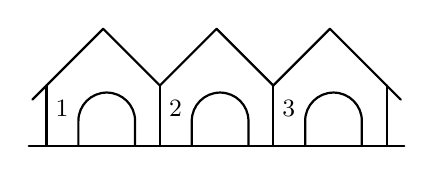
\begin{tikzpicture}[scale=0.9, line cap=round, line join=round, thick]
    % Baseline
    \draw (-0.25, 0) -- (5.05, 0);
    
    % Vertical walls
    \draw (0, 0) -- (0, 0.85);
    \draw (1.6, 0) -- (1.6, 0.85);
    \draw (3.2, 0) -- (3.2, 0.85);
    \draw (4.8, 0) -- (4.8, 0.85);
    
    % Roofs
    % House 1
    \draw (-0.2, 0.65) -- (0.8, 1.65) -- (1.6, 0.85);
    % House 2
    \draw (1.6, 0.85) -- (2.4, 1.65) -- (3.2, 0.85);
    % House 3
    \draw (3.2, 0.85) -- (4.0, 1.65) -- (5.0, 0.65);
    
    % Doors and labels
    % House 1
    \node at (0.22, 0.52) {\small 1};
    \draw (0.45, 0) -- (0.45, 0.35) arc (180:0:0.4) -- (1.25, 0);
    
    % House 2
    \node at (1.82, 0.52) {\small 2};
    \draw (2.05, 0) -- (2.05, 0.35) arc (180:0:0.4) -- (2.85, 0);
    
    % House 3
    \node at (3.42, 0.52) {\small 3};
    \draw (3.65, 0) -- (3.65, 0.35) arc (180:0:0.4) -- (4.45, 0);
  \end{tikzpicture}
  \end{center}
\end{enumerate}
% ==============================================================================
% § IV-2 條件機率與獨立事件
% ==============================================================================
\subsection{條件機率與獨立事件}\label{sec:b5-4-2}

\subsubsection*{甲、條件機率}

設 $(S, P)$ 是一個有限機率空間，以及 $A$ 是其中的一個非空事件，我們現在想討論在假設事件 $A$ 出現的條件之下，任一事件 $B$ 出現的機率，首先請大家看看下面的例子．

\medskip
\noindent\textbf{【論例 4】}某校有已婚男老師25人，已婚女老師25人，未婚男老師15人，未婚女老師10人，在全體老師中任意推選一人擔任福利委員（設各人當選的機會均等）．假設推選結果是一位未婚老師，試求未婚女老師當選的機率．

\indent\textbf{解}\quad 顯然所求機率爲未婚女老師人數與未婚老師人數的比，等於
\[
\frac{10}{15+10} = \frac{2}{5}.
\]
現在我們要對這個答案作進一步的分析，以導出一般的結果．令樣本空間 $S=$ 全體老師的集合，$|S|=25+25+15+10=75$．事件 $A$ 表示未婚老師當選的事件：
\[
A = \text{未婚老師的集合}, \quad |A| = 15+10 = 25.
\]
事件 $B$ 表示女老師當選的事件：
\[
B = \text{女老師的集合}, \quad |B| = 25+10 = 35.
\]
則積事件 $A \cap B$ 表示未婚女老師當選的事件：
\[
A \cap B = \text{未婚女老師的集合}, \quad |A \cap B| = 10.
\]
此時論例 4 中所求的機率卽爲
\[
\frac{2}{5} = \frac{|A \cap B|}{|A|} = \frac{|A \cap B|/|S|}{|A|/|S|} = \frac{P(A \cap B)}{P(A)} = \frac{10/75}{25/75}.
\]
上式表示所求之機率爲 $|A \cap B|$ 與 $|A|$ 之比，亦卽 $A \cap B$ 與 $A$ 二事件的機率之比．這是在機會均等的情形，可以用元素個數的比來討論．

在一般情形，各基本事件的機率不等，就不能利用元素個數計算，但是所求機率仍應等於 $A \cap B$ 與 $A$ 的機率的比．

設 $(S, P)$ 是一個任意的有限機率空間：
\begin{align*}
\text{樣本空間}\quad & S = \{a_1, \dots\dots, a_n\} \\
\text{機率函數}\quad & P : a_j \longmapsto \alpha_j, \quad j = 1, 2, \dots\dots, n. \\
& 0 < \alpha_j \le 1, \quad\text{且}\quad \alpha_1 + \dots\dots + \alpha_n = 1.
\end{align*}
若 $A$ 爲一非空事件，$A=\{a_{k_1}, \dots\dots, a_{k_r}\}$，$0 < r \le n$，則 $P(A) = P(a_{k_1}) + \dots\dots + P(a_{k_r})$．考慮在假設事件 $A$ 出現的條件之下，任一事件 $B$ 出現的機率，記作 $P(B|A)$．顯然我們有
\[
P(A|A) = 1, \quad P(A'|A) = 0 \quad (A' = S - A).
\]
如果 $a' \in A'$，則亦有 $P(a'|A) = 0$．但是如果 $a_{k_j} \in A$，則 $0 < P(a_{k_j}|A) \le 1$，並且
\begin{equation}\tag{1}\label{eq:b5-4-1}
1 = P(A|A) = P(a_{k_1}|A) + \dots\dots + P(a_{k_r}|A)
\end{equation}
其次，$A$ 中各基本事件 $a_{k_j}$ 在假設 $A$ 出現的條件下的機率仍應保持原來的比例：
\begin{equation}\tag{2}\label{eq:b5-4-2}
\frac{P(a_{k_1}|A)}{P(a_{k_1})} = \frac{P(a_{k_2}|A)}{P(a_{k_2})} = \dots\dots = \frac{P(a_{k_r}|A)}{P(a_{k_r})} = K
\end{equation}
（注意，由 §IV-1 中 (7) 式可知 $P(a_{k_i}) > 0, i = 1, \dots\dots, r$）

由 (1), (2) 兩式求得
\[
K = \frac{1}{P(a_{k_1}) + \dots\dots + P(a_{k_r})} = \frac{1}{P(A)},
\]
因此
\begin{equation}\tag{3}\label{eq:b5-4-3}
P(a_{k_j}|A) = \frac{P(a_{k_j})}{P(A)}, \quad j = 1, 2, \dots\dots, r.
\end{equation}
若 $B$ 爲 $S$ 中任一事件，由於 $B = (B \cap A) \cup (B \cap A')$，則
\begin{align*}
P(B|A) &= \sum_{b \in B \cap A} P(b|A) + \sum_{b \in B \cap A'} P(b|A) \\
&= \sum_{b \in B \cap A} P(b|A) = \sum_{b \in B \cap A} \frac{P(b)}{P(A)} \\
&= \frac{1}{P(A)} \sum_{b \in B \cap A} P(b),
\end{align*}
卽
\[
P(B|A) = \frac{P(B \cap A)}{P(A)}.
\]
綜合以上的討論，我們給予條件機率的定義如下：

\medskip
\noindent\textbf{定義}\quad 設 $(S, P)$ 爲一有限機率空間，$A$ 爲任一非空事件．對於任一事件 $B$，我們定義在事件 $A$ 出現之下，事件 $B$ 的條件機率爲
\begin{equation}\tag{4}\label{eq:b5-4-4}
P(B|A) = \frac{P(B \cap A)}{P(A)}
\end{equation}
（顯然此定義爲第三章 §III-1 直觀機率中條件機率的擴展）

這樣所定義的條件機率顯然滿足下列性質：
\begin{enumerate}[label=\Roman*., itemsep=2pt, topsep=2pt]
  \item $0 \le P(B|A) \le 1$．
  \item $P(A|A) = 1$，\quad $P(\phi|A) = 0$．
  \item 若二事件 $B_1, B_2 \subset S$；$B_1 \cap A \neq \phi$，$B_2 \cap A \neq \phi$，則
  \[
  P(B_1 \cup B_2|A) = P(B_1|A) + P(B_2|A) \iff (B_1 \cap A) \cap (B_2 \cap A) = \phi.
  \]
\end{enumerate}

如果我們把 $A$ 看作樣本空間，則由上面這些性質可知條件機率 $P(\,\cdot\,|A)$ 就是 $A$ 上的一個機率函數．因此 $(A, P(\,\cdot\,|A))$ 成爲一個機率空間．

\medskip
\noindent\textbf{〔例 6〕}擲一枚公正的硬幣三次，令 $A$ 表示第一次出現正面的事件，$B$ 表示三次中至少兩次爲正面的事件，試求 $P(B|A)$ 及 $P(A|B)$．

\indent\textbf{解}\quad 由於 $P(A) = \frac{1}{2}$，$P(B) = C_2^3 \left(\frac{1}{2}\right)^3 + C_3^3 \left(\frac{1}{2}\right)^3 = \frac{1}{2}$，
\[
P(A \cap B) = \frac{1}{2}\left[ C_1^2 \left(\frac{1}{2}\right)^2 + C_2^2 \left(\frac{1}{2}\right)^2 \right] = 3/8.
\]
因此
\[
P(B|A) = \frac{P(B \cap A)}{P(A)} = 3/4, \quad P(A|B) = \frac{P(A \cap B)}{P(B)} = 3/4. \tag*{\#}
\]

\medskip
\noindent\textbf{〔例 7〕}擲一粒公正的骰子兩次，令 $A$ 表示第一次出現偶數的事件，$B_7, B_8, B_9$ 分別表示兩次共出現 $7, 8, 9$ 點的事件．求 $P(B_7|A)$，$P(B_8|A)$，$P(B_9|A)$，$P(A|B_7)$，$P(A|B_8)$ 及 $P(A|B_9)$．

\indent\textbf{解}\quad
\begin{align*}
&P(A) = \frac{1}{2}, \quad P(B_7) = \frac{1}{6}, \quad P(B_8) = \frac{5}{36}, \\
&P(B_9) = \frac{1}{9}, \quad P(A \cap B_7) = \frac{1}{12}, \quad P(A \cap B_8) = \frac{1}{12}, \\
&P(A \cap B_9) = \frac{1}{18}.
\end{align*}
因此
\begin{align*}
&P(B_7|A) = \frac{1}{6}, \quad P(B_8|A) = \frac{1}{6}, \\
&P(B_9|A) = \frac{1}{9}, \quad P(A|B_7) = \frac{1}{2}, \quad P(A|B_8) = \frac{3}{5}, \\
&P(A|B_9) = \frac{1}{2}. \tag*{\#}
\end{align*}

\medskip
\noindent\textbf{【論例 5】}設甲袋中有藍球3個，白球5個；乙袋中有藍球2個，白球1個，紅球2個．先依均等機會選出甲袋或乙袋，再依均等機會自選出之袋中取出一球，求取出藍球之機率．

\indent\textbf{解}\quad 我們可作下列樹枝圖
\begin{center}
\begin{tikzpicture}[x=1cm, y=1cm, line width=0.8pt]
  % Apex
  \coordinate (root) at (0, 2.0);
  \coordinate (A) at (-2.0, 1.0);
  \coordinate (B) at (2.0, 1.0);

  \draw (root) -- (-2.0, 1.35) node[midway, above left=-1pt] {$1/2$};
  \draw (root) -- (2.0, 1.35) node[midway, above right=-1pt] {$1/2$};
  \node at (A) {甲};
  \node at (B) {乙};

  % Branches from A
  \coordinate (A_start) at (-2.0, 0.65);
  \coordinate (A_blue) at (-3.2, -0.5);
  \coordinate (A_white) at (-0.8, -0.5);
  \draw (A_start) -- (-3.2, -0.2) node[midway, above left=-1pt] {$3/8$};
  \draw (A_start) -- (-0.8, -0.2) node[midway, above right=-1pt] {$5/8$};
  \node at (A_blue) {藍};
  \node at (A_white) {白};

  % Branches from B
  \coordinate (B_start) at (2.0, 0.65);
  \coordinate (B_blue) at (0.4, -0.5);
  \coordinate (B_white) at (2.0, -0.5);
  \coordinate (B_red) at (3.6, -0.5);
  \draw (B_start) -- (0.4, -0.2) node[midway, above left=-1pt] {$2/5$};
  \draw (B_start) -- (2.0, -0.2) node[pos=0.55, left=3pt] {$1/5$};
  \draw (B_start) -- (3.6, -0.2) node[midway, above right=-1pt] {$2/5$};
  \node at (B_blue) {藍};
  \node at (B_white) {白};
  \node at (B_red) {紅};
\end{tikzpicture}
\end{center}
由此圖看出樣本空間可寫爲：
\[
S = \{\text{甲藍},\, \text{甲白},\, \text{乙藍},\, \text{乙白},\, \text{乙紅}\},
\]
機率函數亦可由上圖得到，因此取出一藍球之機率爲
\[
\frac{1}{2} \cdot \frac{3}{8} + \frac{1}{2} \cdot \frac{2}{5} = \frac{31}{80}.
\]

這個答案可以用條件機率來說明．令取出一藍球之事件爲 $A$，選出甲袋之事件爲 $B$，選出乙袋之事件爲 $C$．因爲 $B \cup C = S$，$B \cap C = \phi$，所以
\[
P(A) = P(A \cap B) + P(A \cap C)
\]
由 (4) 式得
\begin{align*}
P(A \cap B) &= P(A|B) P(B) \\
P(A \cap C) &= P(A|C) P(C).
\end{align*}
代入原式得
\begin{align*}
P(A) &= P(A|B)P(B) + P(A|C)P(C) \\
&= \frac{3}{8} \cdot \frac{1}{2} + \frac{2}{5} \cdot \frac{1}{2} = \frac{31}{80}. \tag*{\#}
\end{align*}

由上面的幾個例子可以看出，普通機率 $P(B)$ 與條件機率 $P(B|A)$ 有時相等，有時不等．

(4) 式可寫爲下列形式
\begin{equation}\tag{$4'$}\label{eq:b5-4-4prime}
P(B \cap A) = P(B|A) P(A)
\end{equation}
($4'$) 式叫做條件機率的乘法公式，一般地，我們有下列定理：

\medskip
\noindent\textbf{*【定理 3】}設 $k$ 爲自然數，$k \ge 2$．若 $A_1, \dots\dots, A_k$ 皆爲非空事件，且 $A_1 \cap \dots\dots \cap A_k \neq \phi$．則
\begin{align}\tag{5}\label{eq:b5-4-5}
P(A_1 \cap \dots\dots \cap A_k) &= P(A_1) P(A_2|A_1) P(A_3|A_1 \cap A_2) \dots\dots \notag \\
&\quad\quad P(A_k|A_1 \cap \dots\dots \cap A_{k-1})
\end{align}
證明與第三章 §III-1 之 (VIII') 的證明相同，故予省略．

\medskip
\noindent\textbf{*〔例 8〕}設一袋中有藍球 8 個，白球 7 個，紅球 5 個，連續採取三次（並設各球被取機會均等）．
\begin{enumerate}[label=(\roman*), itemsep=2pt, topsep=2pt]
  \item 若取出立即放回，求依次取得藍、白、紅球的機率．
  \item 若取出不予放回，求上述事件的機率．
\end{enumerate}

\indent\textbf{解}\quad
( i ) 設第一次取得藍球之事件爲 $A$，第二次取得白球之事件爲 $B$，第三次取得紅球之事件爲 $C$．則所求之機率爲
\[
P(A \cap B \cap C) = P(A) P(B|A) P(C|A \cap B) = \frac{8}{20} \cdot \frac{7}{20} \cdot \frac{5}{20} = \frac{7}{200}.
\]
( ii ) 設各事件同上，則所求之機率爲
\begin{align*}
P(A \cap B \cap C) &= P(A) P(B|A) P(C|A \cap B) \\
&= \frac{8}{20} \cdot \frac{7}{19} \cdot \frac{5}{18} = \frac{7}{171}. \tag*{\#}
\end{align*}

\subsubsection*{乙、貝氏定理}

在本段中我們利用條件機率的概念，導出一個重要而有趣的定理，就是貝氏定理，也叫做貝氏公式，是1763年在貝氏（Thomas Bayes，十八世紀英國牧師）的遺著中所發表．

\medskip
\noindent\textbf{定義}\quad 設 $(S, P)$ 爲有限機率空間；$A_1, \dots\dots, A_r$ 爲非空的互斥事件（卽 $A_i \cap A_j = \phi$ 對於 $i \neq j$），且 $A_1 \cup \dots\dots \cup A_r = S$，我們則稱 $\{A_1, \dots\dots, A_r\}$ 爲樣本空間 $S$ 的一個\textbf{分割}．

\medskip
\noindent\textbf{【定理 4】}設 $\{A_1, \dots\dots, A_r\}$ 爲樣本空間 $S$ 的一個分割，$B$ 爲任意事件，則
\begin{align}\tag{6}\label{eq:b5-4-6}
P(B) &= P(A_1) P(B|A_1) + \dots\dots + P(A_r) P(B|A_r) \notag \\
&= \sum_{j=1}^r P(A_j) P(B|A_j)
\end{align}

\noindent\textbf{證明}\quad 因爲 $\{A_1, \dots\dots, A_r\}$ 爲 $S$ 的一個分割，所以
\[
B = B \cap (A_1 \cup A_2 \cup \dots\dots \cup A_r) = (B \cap A_1) \cup \dots\dots \cup (B \cap A_r),
\]
且 $B \cap A_1, \dots\dots, B \cap A_r$ 亦爲互斥事件．因此由前節定理 1 我們有
\[
P(B) = P(B \cap A_1) + \dots\dots + P(B \cap A_r)
\]
又由 ($4'$) 式，得
\[
P(B) = P(A_1) P(B|A_1) + \dots\dots + P(A_r) P(B|A_r). \tag*{\#}
\]

\begin{center}
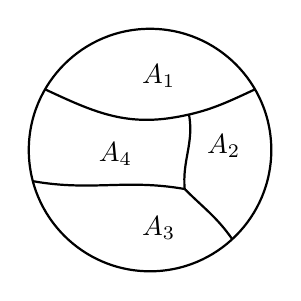
\begin{tikzpicture}[scale=1.1, line width=0.8pt]
  \draw (0,0) circle (1.4);
  % Line 1 (under A1)
  \draw (-1.21, 0.70) to[out=-25, in=190] (0.3, 0.38) to[out=10, in=205] (1.21, 0.70);
  % Line 2 (under A4)
  \draw (-1.35, -0.36) to[out=-10, in=170] (0.4, -0.45);
  % Line 3 (between A4 and A2)
  \draw (0.45, 0.41) to[out=-80, in=95] (0.4, -0.45);
  % Line 4 (between A2 and A3)
  \draw (0.4, -0.45) to[out=-45, in=125] (0.95, -1.03);

  \node at (0.1, 0.85) {$A_1$};
  \node at (-0.4, -0.05) {$A_4$};
  \node at (0.85, 0.05) {$A_2$};
  \node at (0.1, -0.90) {$A_3$};
\end{tikzpicture}
\qquad\qquad
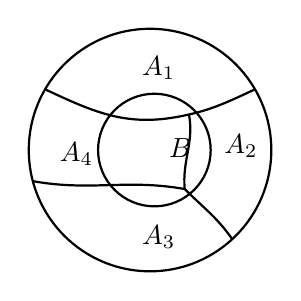
\begin{tikzpicture}[scale=1.1, line width=0.8pt]
  \draw (0,0) circle (1.4);
  % Line 1 (under A1)
  \draw (-1.21, 0.70) to[out=-25, in=190] (0.3, 0.38) to[out=10, in=205] (1.21, 0.70);
  % Line 2 (under A4)
  \draw (-1.35, -0.36) to[out=-10, in=170] (0.4, -0.45);
  % Line 3 (between A4 and A2)
  \draw (0.45, 0.41) to[out=-80, in=95] (0.4, -0.45);
  % Line 4 (between A2 and A3)
  \draw (0.4, -0.45) to[out=-45, in=125] (0.95, -1.03);

  % Event B circle
  \draw (0.05, 0) circle (0.65);

  \node at (0.1, 0.95) {$A_1$};
  \node at (-0.85, -0.05) {$A_4$};
  \node at (1.05, 0.05) {$A_2$};
  \node at (0.1, -1.0) {$A_3$};
  \node at (0.35, 0.02) {$B$};
\end{tikzpicture}
\end{center}

\medskip
\noindent\textbf{〔例 9〕}設有 $r+1$ 個同樣的箱子，編號爲 $0, 1, \dots\dots, r$．在第 $k$ 號箱子有 $k$ 個紅球與 $r-k$ 個綠球（各球形狀相同，只是顏色不同），每箱中皆有 $r$ 個球．先以均等機會選出一箱，自選出的這一個箱連續取 $n$ 次，每次取出記下後立即放回．求連續 $n$ 次全爲紅球的機率，以及第 $n+1$ 次也取到紅球的機率．

\indent\textbf{解}\quad 設任意選出一箱，在其中連續取出（每次立即放回）$n$ 個紅球\phantomsection\label{note:b5-ch4-ex9-ge}\footnote{【原書註記/校訂】：原書作「$n$ 紅球」，語意為「$n$ 個紅球」，此處依現代中文語法補「個」字以臻通順。}的事件爲 $A$，第 $n+1$ 次取得紅球之事件爲 $B$．則所求之機率爲 $P(A)$ 及 $P(B|A)$．再設任意選出第 $k$ 箱的事件爲 $C_k$，顯然 $\{C_0, C_1, \dots\dots, C_r\}$ 是樣本空間的一個分割，因此由定理 4
\begin{align*}
P(A) &= \sum_{k=0}^r P(C_k) P(A|C_k) = \sum_{k=0}^r \frac{1}{r+1} \left(\frac{k}{r}\right)^n = \sum_{k=1}^r \frac{1}{r+1} \left(\frac{k}{r}\right)^n \\
&= \frac{1^n + 2^n + \dots\dots + r^n}{r^n(r+1)},
\end{align*}
同理得
\[
P(A \cap B) = \frac{1^{n+1} + 2^{n+1} + \dots\dots + r^{n+1}}{r^{n+1}(r+1)},
\]
利用 (4) 式則
\[
P(B|A) = \frac{P(A \cap B)}{P(A)} = \frac{1^{n+1} + 2^{n+1} + \dots\dots + r^{n+1}}{r(1^n + 2^n + \dots\dots + r^n)}. \tag*{\#}
\]

\medskip
\noindent\textbf{〔例 10〕}橋藝社由智、仁、勇三班同學組成，各佔 $40\%, 30\%, 30\%$．社員中智班人數的 $1/5$，仁班的 $1/5$，勇班的 $1/3$ 亦爲籃球校隊隊員．某次橋藝社推選新社長，每人當選機會均等，試求籃球隊員當選之機率．

\indent\textbf{解}\quad 設智、仁、勇班同學當選之事件分別爲 $A_1, A_2, A_3$，籃球隊員當選之事件爲 $B$．則
\begin{align*}
P(B) &= P(A_1) P(B|A_1) + P(A_2) P(B|A_2) + P(A_3) P(B|A_3) \\
&= \frac{40}{100} \cdot \frac{1}{5} + \frac{30}{100} \cdot \frac{1}{5} + \frac{30}{100} \cdot \frac{1}{3} = \frac{24}{100}. \tag*{\#}
\end{align*}

\medskip
\noindent\textbf{【定理 5】貝氏定理}

設 $\{A_1, \dots\dots, A_r\}$ 是樣本空間 $S$ 的一個分割，$B$ 是任意非空事件．則對於每個自然數\phantomsection\label{note:b5-ch4-bayes-typo}\footnote{【原書註記/校訂】：原書作「則每對於個自然數 $k$」，疑為「則對於每個自然數 $k$」之字序倒錯，此處予以校正。} $k$，$1 \le k \le r$，我們有
\begin{equation}\tag{7}\label{eq:b5-4-7}
P(A_k|B) = \frac{P(A_k) P(B|A_k)}{\sum_{j=1}^r P(A_j) P(B|A_j)}
\end{equation}

\noindent\textbf{證明}\quad 由條件機率的定義及 ($4'$) 式得
\[
P(A_k|B) = \frac{P(B \cap A_k)}{P(B)} = \frac{P(A_k) P(B|A_k)}{P(B)},
\]
再將分母 $P(B)$ 以 (6) 式代入卽得 (7) 式．\hfill\#

\medskip
\noindent\textbf{〔例 11〕}某燈泡公司有北、中、南三廠，產量比率爲 $30\%, 30\%, 40\%$，各廠產品不合格的比率依次爲 $1.5\%, 1.2\%, 1\%$．某次在總倉庫中任意抽查產品一個，經檢驗爲不合格，求此燈泡爲北廠出品之機率．

\indent\textbf{解}\quad 設抽出爲不合格的事件爲 $B$，抽出爲北、中、南三廠出品的事件依次爲 $A_1, A_2, A_3$．則所求機率爲
\begin{align*}
P(A_1|B) &= \frac{P(A_1) P(B|A_1)}{\sum_{j=1}^3 P(A_j) P(B|A_j)} \\
&= \frac{0.3 \times 0.015}{0.3 \times 0.015 + 0.3 \times 0.012 + 0.4 \times 0.01} = 45/121. \tag*{\#}
\end{align*}

\medskip
\noindent\textbf{〔例 12〕}某項胸部 $X$ 光檢查的可靠程度如下：
\begin{quote}
對於有結核病者，$90\%$ 可發現，$10\%$ 未發現．對於無結核病者，$99\%$ 爲正確，$1\%$ 不正確．設某地區廣大人口中患結核病者佔 $0.1\%$，若其中任意一人經 $X$ 光檢驗有結核病嫌疑，求此人確有結核病的機率．
\end{quote}

\indent\textbf{解}\quad 設 $A$ 表示被選出者有結核病的事件，則 $A'$ 表示無結核病的事件，再設 $B$ 表示檢查有結核病嫌疑的事件．則
\begin{align*}
P(A|B) &= \frac{P(A) P(B|A)}{P(A) P(B|A) + P(A') P(B|A')} \\
&= \frac{0.001 \times 0.9}{0.001 \times 0.9 + 0.999 \times 0.01} = \frac{90}{1089} = 0.083(\text{近似值}). \tag*{\#}
\end{align*}
% ==============================================================================
% 丙、獨立事件
% ==============================================================================
\subsubsection*{丙、獨立事件}\label{sec:b5-4-2-c}

在本節甲段中我們看到，一個事件 $B$ 的機率 $P(B)$ 與條件機率 $P(B\mid A)$，有時相等，有時不等．我們現在要來討論相等的情形．

\medskip
\noindent\textbf{定義}\quad 設 $(S, P)$ 為機率空間，$A, B$ 皆為非空事件．若
\begin{equation}
P(B\mid A) = P(B) \tag{8}\label{eq:b5-4-8}
\end{equation}
成立，則稱 $B$ 與 $A$ \textbf{無關}．

由條件機率定義
\[
P(B\mid A) = \frac{P(B \cap A)}{P(A)}
\]
若 $B$ 與 $A$ 無關，則得
\begin{equation}
P(B) = \frac{P(B \cap A)}{P(A)}. \tag{9}\label{eq:b5-4-9}
\end{equation}
將上式改寫為
\[
P(A) = \frac{P(B \cap A)}{P(B)},
\]
而上式右邊即 $P(A\mid B)$，我們得到
\[
P(A\mid B) = P(A)
\]
表示 $A$ 亦與 $B$ 無關．因此我們進一步給予下列定義．

\medskip
\noindent\textbf{定義}\quad 設 $A, B$ 為非空事件，若 \eqref{eq:b5-4-8} 式成立，則稱 $A, B$ 為\textbf{獨立事件}，否則稱為\textbf{相依事件}．

由 \eqref{eq:b5-4-9} 式我們得到下列定理．

\medskip
\noindent\textbf{【定理 6】（乘法定理）}

設 $A, B$ 為非空事件，則 $A, B$ 為獨立事件的充分必要條件為下列乘法公式成立
\begin{equation}
P(A \cap B) = P(A)P(B) \label{eq:b5-4-10}\tag*{(10)\quad\#}
\end{equation}

\medskip
\noindent\textbf{〔例 13〕}
\begin{enumerate}[(i), leftmargin=2.5em, itemsep=0.3em]
  \item 擲一枚公正的硬幣二次．令 $A$ 表示第一次出現正面的事件，$B$ 表示第二次出現正面的事件．證明 $A, B$ 為獨立事件．
  \item 若令 $A$ 表示至少出現一次正面的事件，$B$ 表示正，反面各出現一次的事件，$A, B$ 是否為獨立事件？
\end{enumerate}

\noindent\textbf{解}
\begin{enumerate}[(i), leftmargin=2.5em, itemsep=0.3em]
  \item $A, B$ 二事件顯然為獨立事件，驗證如下：
  \[
  P(A) = \frac{1}{2}, \quad P(B) = \frac{1}{2}, \quad P(A \cap B) = \frac{1}{4}.
  \]
  所以 $P(A \cap B) = P(A)P(B)$．
  \item $P(A) = 3/4$，$P(B) = 1/2$，$P(A \cap B) = 1/2$．
  
  所以 $P(A \cap B) \neq P(A)P(B)$，$A, B$ 為相依事件．\hfill\#
\end{enumerate}

\medskip
\noindent\textbf{【定理 7】} 若 $A, B$ 為獨立事件，則下列各對事件亦為獨立事件：
\begin{enumerate}[(i), leftmargin=2.5em, itemsep=0.2em]
  \item $A$ 與 $B'$，
  \item $A'$ 與 $B$，
  \item $A'$ 與 $B'$．
\end{enumerate}

\noindent\textbf{證明}\quad 我們只要證一種情形，其他情形即可直接推得．
\begin{enumerate}[(i), leftmargin=2.5em, itemsep=0.3em]
  \item 因為 $P(A) = P(A \cap B) + P(A \cap B')$，所以
  \begin{align*}
  P(A \cap B') &= P(A) - P(A \cap B) \\
  &= P(A) - P(A)P(B) \\
  &= P(A)[1 - P(B)] = P(A)P(B') \tag*{\#}
  \end{align*}
\end{enumerate}

對於三個非空事件 $A, B, C$，如果其中任意一對都是獨立事件，我們還是不能得到類似的乘法公式．

\medskip
\noindent\textbf{【論例 6】} 袋中有 9 個同樣的球，編為 1 到 9 號．採取一球，取到的球號為 $\{1, 5, 9\}$ 的事件為 $A$，為 $\{2, 5, 8\}$ 的事件為 $B$，為 $\{3, 5, 7\}$ 的事件為 $C$．則得
\[
P(A) = 1/3, \quad P(B) = 1/3, \quad P(C) = 1/3;
\]
\[
P(A \cap B) = P(B \cap C) = P(C \cap A) = 1/9;
\]
\[
P(A \cap B \cap C) = 1/9.
\]
因此 $A$ 與 $B$，$B$ 與 $C$，$C$ 與 $A$ 各為獨立事件，但
\[
P(A \cap B \cap C) \neq P(A)P(B)P(C).
\]

對於獨立事件，我們應該要求乘法公式成立，因此直接定義三個事件的獨立性如下：

\medskip
\noindent\textbf{定義}\quad 設 $A, B, C$ 是三個非空事件，若其中每一對皆為獨立事件，而且乘法公式成立
\[
P(A \cap B \cap C) = P(A)P(B)P(C),
\]
則稱 $A, B, C$ 三事件為\textbf{獨立}．

\medskip
\noindent\textbf{〔例 14〕} 袋中有 120 個同樣的球，編為 1 到 120 號．採取一次，設取出球號為 2 的倍數的事件為 $A$，$3$ 的倍數為 $B$，$5$ 的倍數為 $C$，則 $A, B, C$ 為獨立事件．

\noindent\textbf{證明}\quad
\begin{align*}
P(A) &= 1/2, & P(B) &= 1/3, & P(C) &= 1/5; \\
P(A \cap B) &= 1/6, & P(B \cap C) &= 1/15, & P(C \cap A) &= 1/10; \\
P(A \cap B \cap C) &= 1/30.
\end{align*}
滿足定義的條件．\hfill\#

\medskip
\noindent\textbf{〔例 15〕} 甲、乙、丙三射手同射一靶，每人一發，設甲、乙、丙的射擊命中率各為 $0.5, 0.6, 0.8$，並設皆為有經驗射手，不受他人干擾．問靶面恰中一發的機率是多少？

\noindent\textbf{解}\quad 設甲、乙、丙命中的事件為 $A, B, C$．則由假設 $A, B, C$ 為獨立事件，而
\[
P(A) = 0.5, \quad P(B) = 0.6, \quad P(C) = 0.8.
\]
靶面恰中一發的機率為
\begin{align*}
& P(A \cap B' \cap C') + P(A' \cap B \cap C') + P(A' \cap B' \cap C) \\
&= P(A)P(B')P(C') + P(A')P(B)P(C') + P(A')P(B')P(C) \\
&= 0.5 \times 0.4 \times 0.2 + 0.5 \times 0.6 \times 0.2 + 0.5 \times 0.4 \times 0.8 \\
&= 0.26. \tag*{\#}
\end{align*}

下面我們討論重複進行同一試驗或不同試驗的情形，但假設各個試驗互為獨立，試驗的結果不受影響．

擲骰子一次的機率空間為
\[
S = \{1, 2, 3, 4, 5, 6\},
\]
\[
P(k) = 1/6, \quad k = 1, \dots, 6.
\]
如果擲骰子二次，則可取樣本空間為 $S$ 與 $S$ 的直積：
\[
S \times S = \{(j, k) \mid j, k = 1, 2, \dots, 6\}.
\]
而機率函數應定為
\[
P[(j, k)] = P(j)P(k), \quad j, k = 1, 2, \dots, 6.
\]
這樣就得到擲骰子二次這一試驗的機率空間．

對於一般情形，我們也可仿照這種方法討論．設 $(S, P)$ 為一任意機率空間，$S = \{a_1, \dots, a_n\}$．如將此試驗重複 $k$ 次，而視為一項綜合試驗，則其樣本空間可取為 $S^k = S \times \dots \times S$，而機率函數定為
\[
P^*(A_1 \times \dots \times A_k) = P(A_1) \dots P(A_k),
\]
式中 $A_1 \times \dots \times A_k \subset S^k$ 為一事件．

如果 $A, B \subset S$ 是獨立事件，則由下列計算
\begin{align*}
& P[(A \times \underbrace{S \times \dots \times S}_{k-1}) \cap (B \times S \times \dots \times S)] \\
&= P[(A \cap B) \times S \times \dots \times S] \\
&= P(A \cap B) P(S) \dots P(S) = P(A \cap B) \quad (\because P(S) = 1) \\
&= P(A)P(B) \\
&= [P(A) P(S) \dots P(S)][P(B) P(S) \dots P(S)] \\
&= P(A \times S \times \dots \times S) P(B \times S \times \dots \times S),
\end{align*}
得到 $A \times S \times \dots \times S, B \times S \times \dots \times S \subset S^k$ 亦為獨立事件．又若 $A, B \subset S$ 為任意非空事件，則 $A \times S \times \dots \times S, S \times B \times S \times \dots \times S \subset S^k$ 亦為獨立事件，更進一步，若 $A_1, \dots, A_k \subset S$ 為非空事件，則 $S^k$ 中 $A_1 \times S \times \dots \times S, S \times A_2 \times S \times \dots \times S, \dots, S \times \dots \times S \times A_k$ 為獨立事件．

\medskip
\noindent\textbf{〔例 16〕} 某次測驗有 20 個選擇題，每題有 5 個答案，其中一個是正確的．如果任意猜選，問選對至少 10 題的機率是多少？

\noindent\textbf{解}\quad 答對一題的機率是 $P(\text{對}) = 1/5$，則 $P(\text{錯}) = 4/5$．一題的樣本空間為 $S = \{\text{對}, \text{錯}\}$，20 題的樣本空間則為 $S^{20}$．設答對恰好 $k$ 題的一個基本事件為 $a$，則
\[
P^*(a) = \left(\frac{1}{5}\right)^k \left(\frac{4}{5}\right)^{20-k},
\]
令答對恰好 $k$ 題的事件為 $A_k$，則
\[
P^*(A_k) = C^{20}_k \left(\frac{1}{5}\right)^k \left(\frac{4}{5}\right)^{20-k},
\]
因此至少選對 10 題之機率為
\[
P^*(A_{10}) + \dots + P^*(A_{20}) = \sum_{k=10}^{20} C^{20}_k \left(\frac{1}{5}\right)^k \left(\frac{4}{5}\right)^{20-k}. \tag*{\#}
\]

對於不同的試驗，我們也可以同樣討論．

\medskip
\noindent\textbf{〔例 17〕} 擲公正的硬幣一枚及公正的骰子一粒，則機率空間分別為
\[
S = \{\text{正}, \text{反}\}, \quad P_1(\text{正}) = 1/2, \quad P_1(\text{反}) = 1/2;
\]
\[
T = \{1, 2, 3, 4, 5, 6\}, \quad P_2(k) = 1/6, \quad k = 1, \dots, 6.
\]
若二者合併觀察，則樣本空間為
\[
S \times T = \{(\text{正}, 1), \dots, (\text{正}, 6), (\text{反}, 1), \dots, (\text{反}, 6)\},
\]
機率函數
\[
P^*(\text{正}, k) = P_1(\text{正}) P_2(k) = \frac{1}{2} \cdot \frac{1}{6} = \frac{1}{12},
\]
\[
P^*(\text{反}, k) = P_1(\text{反}) P_2(k) = \frac{1}{2} \cdot \frac{1}{6} = \frac{1}{12}.
\]

\medskip
\noindent
\begin{minipage}[c]{0.56\textwidth}
\noindent\textbf{〔例 18〕} 設有棋盤形街道如下圖．甲由 $A$ 走向 $B$，乙由 $B$ 走向 $A$，二人速度相同，求二人在途中相遇的機率．(設自起點至中點 $C, D, E, F$ 各路線被選取的機會均等)．

\medskip
\noindent\textbf{解}\quad 如果相遇，則在 $C, D, E, F$ 四點之一，故設樣本空間 $S = \{C, D, E, F\}$．
\end{minipage}\hfill
\begin{minipage}[c]{0.40\textwidth}
\centering
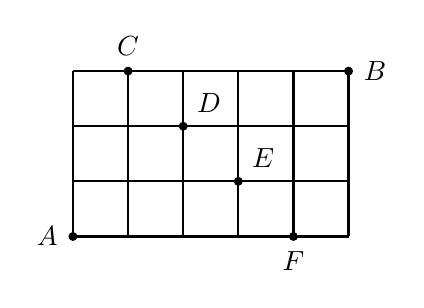
\begin{tikzpicture}[scale=0.7]
  \draw[line width=0.8pt] (0,0) grid (5,3);
  \filldraw[black] (0,0) circle (2pt) node[left=2pt] {$A$};
  \filldraw[black] (5,3) circle (2pt) node[right=2pt] {$B$};
  \filldraw[black] (1,3) circle (2pt) node[above=2pt] {$C$};
  \filldraw[black] (2,2) circle (2pt) node[above right=1.5pt] {$D$};
  \filldraw[black] (3,1) circle (2pt) node[above right=1.5pt] {$E$};
  \filldraw[black] (4,0) circle (2pt) node[below=2pt] {$F$};
\end{tikzpicture}
\par\vspace{0.4em}
{\small 圖 3-1\phantomsection\label{note:b5-ch4-p136-fig-num}\footnote{【原書註記/校訂】：原書圖號作「3-1」，按第四章圖號編次疑應為「圖 4-1」，茲存其舊並予註記說明．}}
\end{minipage}

\medskip
\noindent 甲走到 $C$ 點的走法有 $C^1_4$ 種，至 $D$ 點有 $C^2_4$ 種，至 $E$ 點有 $C^3_4$ 種，至 $F$ 點有 $C^4_4$ 種，共有 $C^1_4 + C^2_4 + C^3_4 + C^4_4 = 15$ 種走法．因此甲走到各點的機率為
\[
P_1(C) = \frac{4}{15}, \quad P_1(D) = \frac{6}{15}, \quad P_1(E) = \frac{4}{15}, \quad P_1(F) = \frac{1}{15}.
\]
乙走到各點的機率則為
\[
P_2(C) = \frac{1}{15}, \quad P_2(D) = \frac{4}{15}, \quad P_2(E) = \frac{6}{15}, \quad P_2(F) = \frac{4}{15}.
\]
因此二人相遇的機率為
\begin{align*}
& P^*(C, C) + P^*(D, D) + P^*(E, E) + P^*(F, F) \\
&= P_1(C)P_2(C) + P_1(D)P_2(D) + P_1(E)P_2(E) + P_1(F)P_2(F) \\
&= \frac{4}{15} \cdot \frac{1}{15} + \frac{6}{15} \cdot \frac{4}{15} + \frac{4}{15} \cdot \frac{6}{15} + \frac{1}{15} \cdot \frac{4}{15} = \frac{56}{225}. \tag*{\#}
\end{align*}

\vspace{1.5em}
% ==============================================================================
% 習題 IV-2
% ==============================================================================
\subsubsection*{習題 IV-2}\label{sec:b5-ex4-2}

\begin{enumerate}[label=\textbf{\arabic*.}]
  \item 重複丟一枚公正的硬幣，令 $B$ 表示首 $n$ 次皆出現反面的事件，$A$ 表示第 $n+1$ 次出現正面的事件，試求 $P(A\mid B)$．
  \item 擲公正的硬幣五次，令 $A$ 表示首兩次出現正面的事件，$B$ 表示五次中至少三次為正面的事件，試求：$P(B\mid A)$ 及 $P(A\mid B)$．
  \item 擲公正的骰子三次，令 $A$ 表示第一次出現偶數的事件，$B_{10}, B_{11}, B_{12}$ 分別表示三次共出現 $10, 11, 12$ 點的事件，試求 $P(B_{10}\mid A), P(A\mid B_{10})$ 等事件機率．
  \item 
  \begin{enumerate}[label=(\arabic*)]
    \item 袋中有 30 個白球及 15 個黑球，若任意採取 10 次（每次球取出不放回），試求在其中恰好取到 6 白球的條件下，最初兩球皆為白球的機率．
    \item 同上題，但改為取出隨即放回．
  \end{enumerate}
  \item 袋中有紅、黃、藍、白四色的球，各種數量相等，若連續採取四次（設各球被取機會均等，取出隨即放回），令 $A$ 表示所取四球有三種不同顏色的事件，$B$ 表示有兩種不同顏色的事件，$C$ 表示其中恰有兩球為紅色的事件，試求：$P(A \cap C), P(B \cap C), P(A\mid C), P(C\mid A), P(B\mid C)$ 及 $P(C\mid B)$．
  \item 自 $\{1, 2, 3, \dots, 100\}$ 中任取一數（設各數被取機會相等），令 $A$ 表示所取為 2 的倍數的事件，$B$ 表示 3 的倍數的事件，$C$ 表示 5 的倍數的事件，試討論相互間的獨立性．
  \item 作例 11，但將不合格的比例依次改為 $1.2\%, 0.9\%, 0.8\%$．
  \item 作例 18，但將橫街改為 5 條，縱街改為 7 條．
\end{enumerate}

\vspace{2em}
% ==============================================================================
% **附錄：一般機率空間的定義
% ==============================================================================
\subsection*{**附錄：一般機率空間的定義}\label{sec:b5-ch4-appendix}

設 $S$ 為一個非空（有限的或無限的）集合，$\mathscr{P}$ 為 $S$ 的全部子集族（即 $S$ 的全部子集所成的集合），以及 $\mathscr{F}$ 為 $S$ 的若干子集所成的一個非空的族，即 $\mathscr{F} \subset \mathscr{P}$，$\mathscr{F} \neq \phi$．如果 $\mathscr{F}$ 滿足
\begin{enumerate}[label=\arabic*)]
  \item 如果 $A \in \mathscr{F}$，則 $A' = S - A \in \mathscr{F}$
  \item 如果 $A_k \in \mathscr{F}, k = 1, 2, \dots$，則
  \[
  A_1, A_2, \dots \text{ 的聯集 } \bigcup_{k=1}^\infty A_k \in \mathscr{F}
  \]
\end{enumerate}
我們則稱 $\mathscr{F}$ 是一個（$S$ 的子集的）$\sigma$-體（$\sigma$ 為希臘字母，唸做 Sigma）．例如 $S$ 的全部子集族 $\mathscr{P}$ 顯然是一個 $\sigma$-體．

設 $\mathscr{F}$ 是一個 $\sigma$-體，我們可以推得
\begin{enumerate}[label=\roman*)]
  \item $S \in \mathscr{F}$ 及 $\phi \in \mathscr{F}$
  \item 若 $A_1, A_2, \dots \in \mathscr{F}$，則 $\ds\bigcap_{k=1}^\infty A_k \in \mathscr{F}$
\end{enumerate}

\noindent\textbf{證明}\quad 因 $\mathscr{F}$ 是一個非空的族，任取 $A \in \mathscr{F}$，由 1) $A' \in \mathscr{F}$，由 2) $A \cup A' = S \in \mathscr{F}$．又由 1) $S' = \phi \in \mathscr{F}$．

設 $A_1, A_2, \dots \in \mathscr{F}$，則由 1) 及 2) 得
\[
\bigcap_{k=1}^\infty A_k = \left( \bigcup_{k=1}^\infty A_k' \right)' \in \mathscr{F}. \tag*{\#}
\]

設 $P$ 為定義在 $S$ 的子集所成的一個 $\sigma$-體，$\mathscr{F}$ 上的一個實數值函數．如果 $P$ 滿足
\begin{enumerate}[label=\arabic*)]
  \item $P(A) \ge 0$ 對於每個 $A \in \mathscr{F}$\phantomsection\label{note:b5-ch4-p138-f-font}\footnote{【原書註記/校訂】：原書此處條件 1) 與 2) 中誤植為普通斜體「$F$」，前後文定義 $\sigma$-體皆用花體「$\mathscr{F}$」，茲統一校訂為「$\mathscr{F}$」．}．
  \item 如果 $A_k \in \mathscr{F}, k = 1, 2, \dots$，且其中任意二集合皆不相交，則
  \[
  P\left( \bigcup_{k=1}^\infty A_k \right) = \sum_{k=1}^\infty P(A_k).
  \]
  \item $P(S) = 1$，
\end{enumerate}
我們則稱 $P$ 為 $S$ 上的\textbf{機率測度} (Probability measure) 或\textbf{機率} (Probability)，而稱 $S$ 為\textbf{樣本空間}，$S$ 中的每個元素 $a$ 為\textbf{樣本點}或\textbf{基本事件}，$\mathscr{F}$ 中每個元素 $A$（即 $S$ 的一個子集）為\textbf{事件}．$S, \mathscr{F}$ 與 $P$ 所成的一組則稱為一個\textbf{機率空間}，記作 $(S, \mathscr{F}, P)$．

在本章中所討論的有限機率空間都是將 $\sigma$-體 $\mathscr{F}$ 取為 $S$ 的全部子集族 $\mathscr{P}$，即 $\mathscr{F} = \mathscr{P}$．依照這裡的定義應記作 $(S, \mathscr{P}, P)$．由於我們只考慮這樣的情形，所以可將其中的 $\mathscr{P}$ 省略，而簡記為 $(S, P)$．雖然我們為了簡便只討論 $\mathscr{F} = \mathscr{P}$ 的情形，但是並沒有失去普遍性．這一點可以概略地由下面的例子看出．

\medskip
\noindent\textbf{〔例〕} 擲一粒公正的骰子，考慮出現奇數點或偶數點的機率．

\noindent\textbf{解}\quad 樣本空間 $S = \{1, 2, 3, 4, 5, 6\}$．令 $A$ 為 $S$ 中奇數的集合，$A = \{1, 3, 5\}$，及 $B$ 為 $S$ 中偶數的集合，$B = \{2, 4, 6\}$．作 $S$ 的子集族 $\mathscr{F} = \{\phi, A, B, S\}$，則 $\mathscr{F}$ 成一 $\sigma$-體．定義 $\mathscr{F}$ 上一個函數 $P$：
\[
P(\phi) = 0, \quad P(A) = P(B) = \frac{1}{2}, \quad P(S) = 1,
\]
則得到一個機率空間 $(S, \mathscr{F}, P)$，其中 $\mathscr{F} \neq \mathscr{P}$．

我們可將 $\mathscr{F}$ 上的函數 $P$ 擴展為 $\mathscr{P}$ 上的函數 $P^*$，即由定義
\[
P^*(C) = \frac{|C|}{6}, \quad C \in \mathscr{P}
\]
得到 $\mathscr{P}$ 上的一個函數 $P^*$，而 $P$ 只是將 $P^*$ 限制在 $\mathscr{F}$ 上的情形．這樣我們得到機率空間
\[
(S, \mathscr{P}, P^*) = (S, P^*).
\]
如將 $P^*$ 限制在 $\mathscr{F}$ 上，即得原來的機率空間 $(S, \mathscr{F}, P)$．

其次，我們也可將機率空間 $(S, \mathscr{F}, P)$ 中的樣本空間簡化為 $S' = \{A, B\}$．$S'$ 的全部子集族則為 $\mathscr{P}' = \{\phi, \{A\}, \{B\}, S'\}$．如在 $\mathscr{P}'$ 上定義函數 $P'$：
\[
P'(\phi) = 0, \quad P'(\{A\}) = P'(\{B\}) = \frac{1}{2}, \quad P'(S') = 1,
\]
則得機率空間 $(S', \mathscr{P}', P') = (S', P')$，而 $(S', P')$ 與 $(S, \mathscr{F}, P)$ 在本質上是相同的．

至於前章中所述幾何機率，我們只是舉例概略介紹．如果要寫出它們的機率空間，則甚為繁難．例如在例 9 $S=\{x \mid 0 \le x \le 1\}$ 中有很多子集，我們不能規定它們的長度，在例 11 的正方形及例 12 的長方形中有很多子集我們不能規定它們的面積\phantomsection\label{note:b5-ch4-p139-geom-ex-num}\footnote{【原書註記/校訂】：原書此處作「例 9」、「例 11」與「例 12」，核對第三章 *§ III-3 幾何機率之例題，實數區間 $[0,1]$ 為〔例 10〕，約會問題之正方形區域為〔例 12〕，擲針問題之長方形區域為〔例 13〕．疑編著者引用早期初稿編號所致，此處存其舊並予註記說明．}．因此我們不能取 $\mathscr{F} = \mathscr{P}$，而必須應用此附錄中一般機率空間的定義．
